% -*- TeX-master: "main.tex" -*-

\chapter*{Abstract}
\fixme{}

\chapter*{Management Summary}
\section*{Introduction}
The qutebrowser project is a web browser, comparable to Google Chrome or Mozilla
Firefox, which is focused on being keyboard-driven and having a minimal user
interface. It is aimed at power-users who value customizability and efficiency,
but are willing to accept a rather steep learning curve compared to
``traditional'' web browsers.

Since qutebrowser uses the Python programming language in conjunction with the
Qt library for graphical user interfaces, it is standing on the shoulders of
giants: It does not implement complex tasks such as downloading and executing
HTML/CSS/JavaScript code itself. Instead, it relies on the QtWebEngine project
to so, which is largely based on the same code as Google Chrome.

Work on qutebrowser started in December 2013. Since then, it gained a big
community of thousands of users and dozens of contributors. The aim of this
research project is to separate functionality implemented in qutebrowser into a
core and various extensions.

\begin{figure}[H]
  \centering
  
\includegraphics[width=0.7\linewidth]{img/logos.pdf}
  \caption{Technologies used}
\end{figure}

\section*{Objective}

In contrast to Chrome and Firefox, qutebrowser does not support extending its
functionality via extensions. Over its lifetime, various features have been
added to its core by its maintainer (who is the author of this report) and its
contributors. However, this caused its core to grow substantially, getting more
and more complex over time.

Many users of qutebrowser are power-users and, as such, have very specific (and
sometimes unique) feature requests and workflows. It should be possible for
those users to extend qutebrowser with custom extensions in an easy way, in
order to keep qutebrowser's core small and simple.

The goal of this project was to make qutebrowser extensible, by introducing a
clearly defined programming interface (API) which can be used to develop
extensions.

Since qutebrowser already has a thriving community, this change also intends to
decentralize development efforts, as it enables users and developers to maintain
their extensions independently from qutebrowser's core development.

\begin{figure}[H]
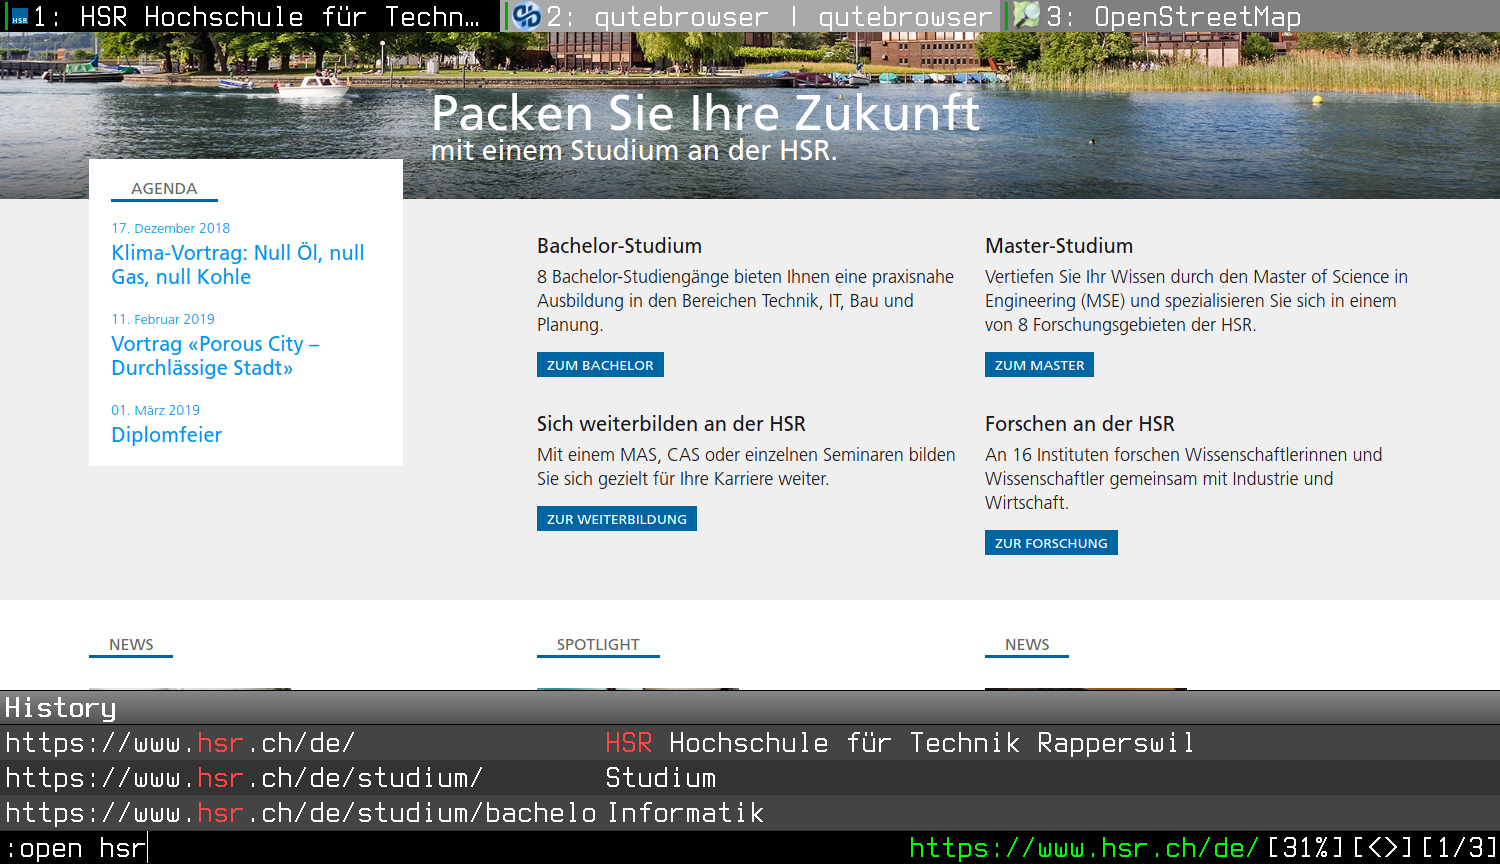
\includegraphics[width=\linewidth]{img/screenshot-intro.png}
\caption{qutebrowser displaying its history completion}
\end{figure}

\section*{Procedure / Results}
Before attempting to expose an interface for extensions from qutebrowser,
various problematic areas in qutebrowser's codebase had to be cleaned up due to
``technical debt'' accumulating in the past. Subsequently, functionality
suitable for moving out of the core into extensions was identified. Based on
the selected areas of code, a concept for an extension API\footnote{Application
programming interface} was developed. After implementing said API in
qutebrowser, large parts of functionality (such as the adblocker, blocking
advertisements on websites) could be moved into extensions. The resulting
changes increased code maintainability and simplicity.

In order to further follow best practices in the software development world,
tools for checking data types (thus reducing the chance of accidental software
defects) were evaluated. The \emph{mypy} tool is now run regularly over
qutebrowser's code, which resulted in various lingering defects being found in
qutebrowser itself and in related projects. Important parts of qutebrowser were
annotated with type information in order to find such issues, also serving as
additional developer documentation.

\section*{Future Work}
This research project was focused on increasing qutebrowser's software quality
and moving parts of its core into extensions. As a next step, additional
functionality should be exposed to extensions, allowing more code to be moved
out of the core.

When the exposed interfaces are expected to be reasonably stable,
they should then be gradually opened to interested external developers so that
third-party extensions can be written.

After third-party extensions gain enough traction, an ``extension manager''
should be developed, so that users can easily install and update available
extensions via a graphical interface.